\documentclass{article}
\usepackage[T1]{fontenc}
\usepackage{lmodern}
\usepackage{graphicx}
\usepackage{amsmath,amssymb}
\usepackage[a4paper,margin=2cm]{geometry}
\usepackage[absolute,overlay]{textpos}
\setlength{\TPHorizModule}{1mm}
\setlength{\TPVertModule}{1mm}
\usepackage[indonesian]{babel}
\usepackage{hyperref}
\setlength{\emergencystretch}{2em}
% unit: Halaman 33

\begin{document}

% === Halaman 33 (llm) ===

% (tidak ada teks dari model)

% deskripsi: Kolase gambar yang menunjukkan lukisan klasik suasana pesta atau kerumunan orang yang sebagian permukaannya tampak terkelupas atau terlipat, mengungkap latar belakang hitam putih yang abstrak di bawahnya.
% bbox normalisasi: [0.2600, 0.1500, 0.7670, 0.8030]
\begin{textblock*}{106.47mm}(54.60mm,44.55mm)
\noindent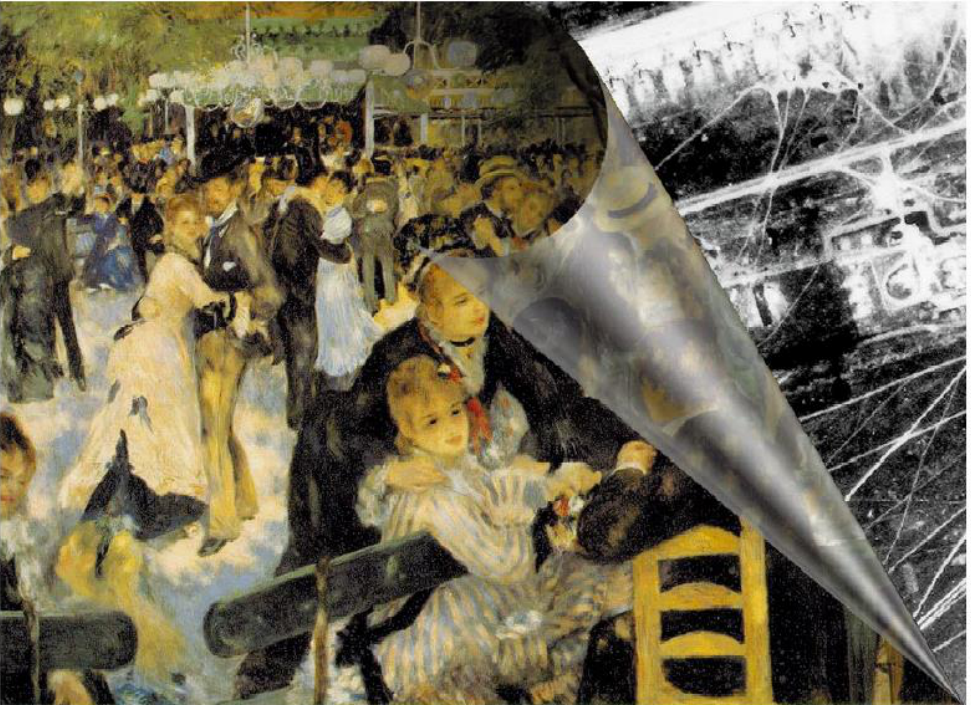
\includegraphics[width=106.47mm,height=193.94mm]{../../images/llm/page_033_img_01.png}%
\end{textblock*}

\end{document}
